\chapter{彩虹表算法优化设计与实现}
\section{计算能力优化}
	\subsection{基于GPU的优化方案}
	\subsection{基于云计算的优化方案}
\section{存储优化}
对于时空折中算法而言,除了要对时间进行优化,还有对空间进行优化,在不增加(或增加少量)时间代价的前提,如何减小空间代价,这就需要我们对系统进行存储优化。我们将从两方面进行改进。第一,针对存储的文件优化,也就是彩虹表文件,我们将设计一个新型的彩虹表存储结构体,减少彩虹表的磁盘存储空间,缩小系统读取文件的时间,从而提升破解的速度;第二,优化存储系统,如采用适合大文件的文件系统,采用快速的物理存储设备等方面提升读取速度。

从上一章彩虹表磁盘空间占用公式\eqref{equ:4.2}可知,想要覆盖更大的密钥空间要么增加彩虹链数或者彩虹表的张数,这都回产生庞大的彩虹表文件,可能会达到几百个GB,甚至上TB的文件,这将会增加大量的文件读取时间和磁盘空间,因此对表的存储结构进行优化将十分有必要。我们将新设计的彩虹链,在以前的存储结构中我们是使用了一个64比特的非负整形变量定义开始节点,而在实际当中,我们并不需要这么大的节点,比如在第四章中的ntlm的彩虹表中,我们只定义了26比特的开始节点和30比特的末端节点,这样一条彩虹链所占用的字节数为7Bytes。代入公式\eqref{equ:4.2}可以得到一张优化后的表的大小为448MB,优化了56.25\%。这样大大减小系统的存储空间和读取文件的时间。
\begin{figure}[!ht]
\centering
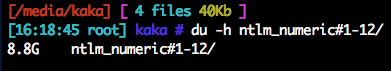
\includegraphics[scale=1]{5-1.png}
\caption{优化后彩虹表的空间大小}
\label{fig:5.1}
\end{figure}

新的彩虹链的数据结构实现如下,在以后的测试实验中,我们将都采用这种优化过的彩虹表。
\begin{lstlisting}
struct RTCFileHeader
{
    unsigned int   uVersion;    
    unsigned short uIndexSBits; 
    unsigned short uIndexEBits; 
    uint64         uIndexSMin;
    uint64         uIndexEMin;
    uint64         uIndexEInterval;
};
\end{lstlisting}

在存储上,除了对表的大小进行优化,还可以对系统的储存架构进行优化。在文件系统上,我们采用先进的XFS文件系统,XFS是由Silico Graphics,Inc.于90年代初开发的,它采用了优化算法,对查询分配存储空间非常快,可以支持上百万T字节的存储空间,特别是对大文件的支持表现相当出众;XFS采用B+树结构保证文件系统可以快速搜索于空间分配;XFS几乎以接近裸设备I/O的性能存储数据,在单个文件系统测试种,其吞吐量可高达7GB每秒,对单个文件的读写操作,其吞吐量可达4GB每秒。基于XFS以上特性,正符合彩虹表多个大文件读取的特点,下图为XFS与EXT3、EXT4的性能比较:
\begin{figure}[!ht]
\centering
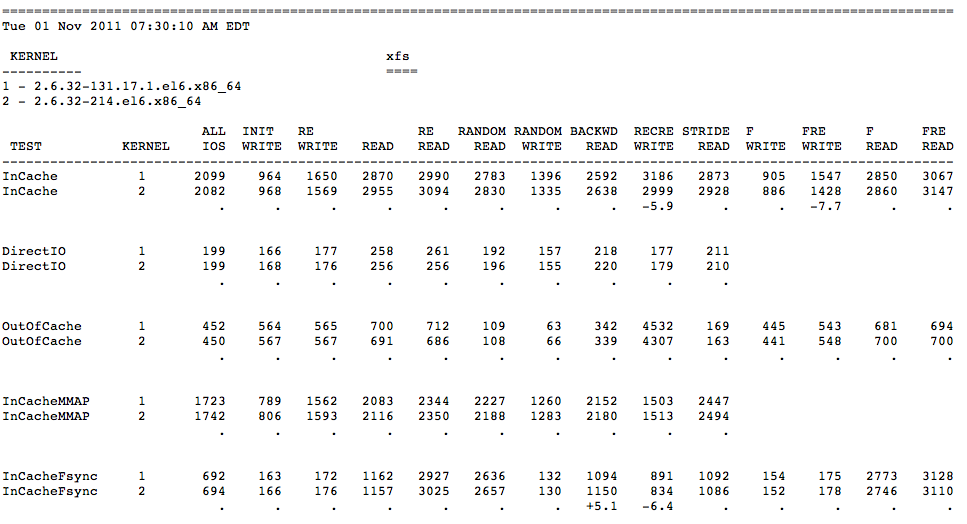
\includegraphics[scale=0.35]{5-2.png}
\caption{XFS性能测试}
\label{fig:5.2}
\end{figure}
\begin{figure}[!ht]
\centering
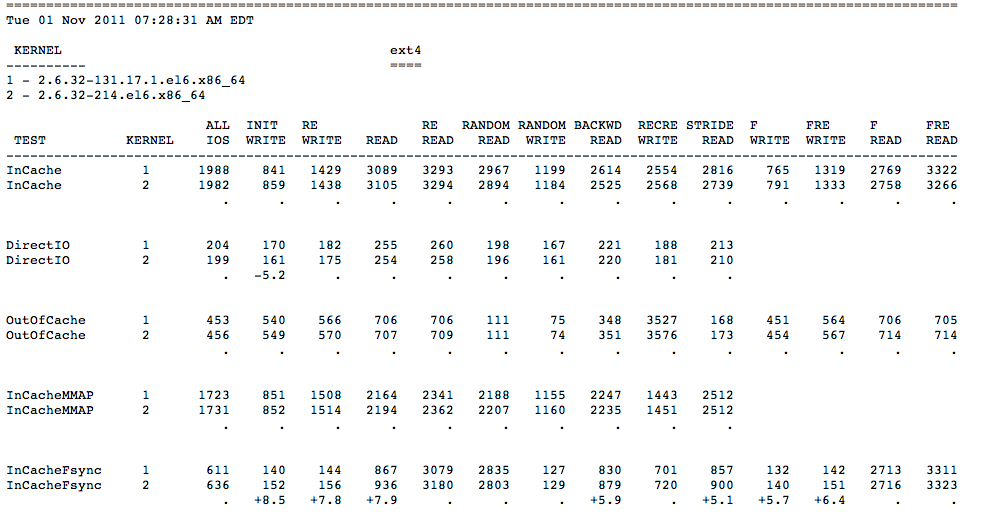
\includegraphics[scale=0.35]{5-3.png}
\caption{EXT4性能测试}
\label{fig:5.3}
\end{figure}
\begin{figure}[!ht]
\centering
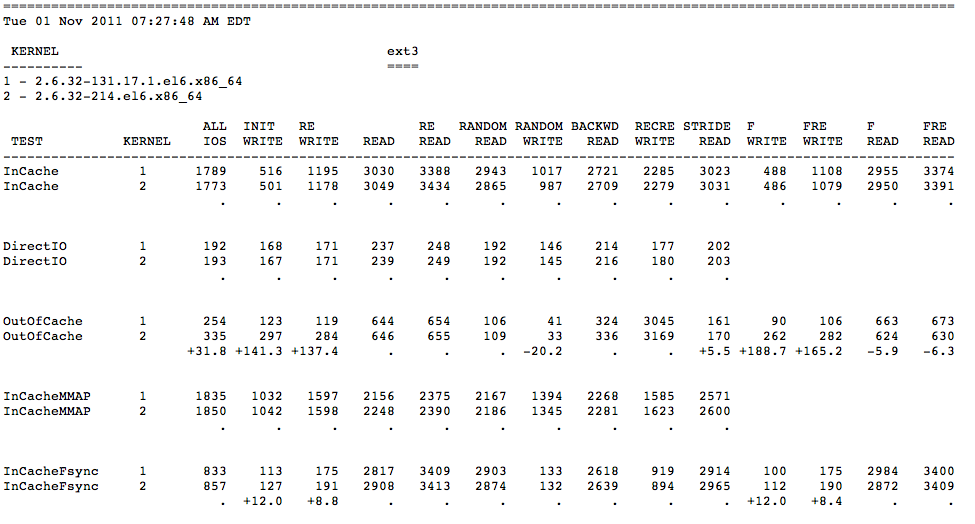
\includegraphics[scale=0.35]{5-4.png}
\caption{EXT3性能测试}
\label{fig:5.4}
\end{figure}
从这3组性能测试数据我们可以看出XFS在大多数的的选项上要优于EXT4和EXT3,特别是在大文件的读取上。

接着是升级磁盘,表是我们对不同的硬盘的读速度进行对比
最后的升级是增加系统内存,在Linux系统上内存以/dev/shm/设备呈现给用户,用户可以对次进行读写操作。
\section{算法结构优化}
\section{本文的实现与性能分析}
